%!TEX root = ../masters_thesis.tex

\chapter{Development} % (fold)
\label{cha:development}

The aim of this thesis is to create a Historical Geographic Information System to visualize and edit the evolution of countries in time and space. This is a complicated task, because both the reality and the human using the system are complex. For such complex applications the methodologies of \emph{Human Centered Design} are promising to create an interface that humans can easily understand.

The development process is iterative and divided in several phases. In each phase creates a prototype or the interface that gets closer to the final solution by increasing the fidelity of the prototype. A phase starts with an initial set of requirements. In multiple iterations, a prototype is developed that solves the problem. Each iteration has four steps: The requirements for the system are analyzed in the \emph{planning} step. Afterwards, they translated into an abstract \emph{design} which is realized in a specific \emph{implementation} of the prototype. Finally, this prototype is tested with humans to find out how well it works. Based on the results of this \emph{testing} step, the requirements are updated and the next iteration starts. This is repeated until a version of the interface is created that sufficiently solves the problem. Then the fidelity is increased, starting the next development phase. The five phases in this thesis are shown in figure \ref{fig:hcd}.

\begin{figure}[H]
  \vspace{1em}
  \centering
  \includegraphics[width=0.9\textwidth]{graphics/development/hcd}
  \caption{Human Centered Design process with five project phases}
  \label{fig:hcd}
\end{figure}

\newpage
\begin{compactenum}
  \item \textbf{Idea}: The initial idea how to edit and visualize the history of countries.
  \item \textbf{Paper Prototype}: The concept of the interface realized and tested on paper.
  \item \textbf{Mockup Prototype}: The concrete workflow developed in a slide-based presentation.
  \item \textbf{Web-Based Prototype}: The final version developed in a Web application.
  \item \textbf{Extensions}: Design approaches to account for the uncertain nature of history.
\end{compactenum}

There are several models involved in the development of the software, each of them has to be developed or analyzed separately. The \emph{data model} is an abstraction and simplification of the real world. The \emph{Hivent Model} developed in this thesis is explained in the first section \ref{sec:hivent_model} of this chapter. It follows the method to \emph{edit} the spatio-temporal data in the system in section \ref{sec:editing_hivent_data}. In iteractive computer systems, the \emph{mental model} is the representation in the mind of the human about how the interface should work -- the \emph{conceptual model} describes the way the interface actually works. The goal of Human Centered Design is to match the conceptual model to the mental model. Section \ref{sec:user_interface_design_process} outlines the gradual design process to reach this goal. In the application, the data model is implemented in the \emph{database model}. The task for the \emph{computational model} is to translate between the database model and the conceptual model. The HistoGlobe application, including the database and computational model, is introduced in the last section \ref{sec:application} of this chapter.

\begin{figure}[H]
  \vspace{1em}
  \centering
  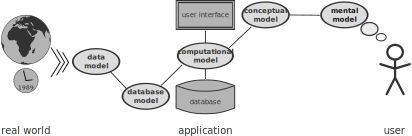
\includegraphics[width=0.8\textwidth]{graphics/development/models}
  \caption{Relevant models for an information system}
  \label{fig:models}
\end{figure}

% ==============================================================================
%!TEX root = ../masters_thesis.tex

\section{Hivent Model} % (fold)
\label{sec:hivent_model}

This section proposes the spatio-temporal \emph{Hivent model} to represent the history of countries in time and space. \emph{Hivent} is an acronym for \emph{\textbf{Hi}}storical e\emph{\textbf{vent}} and is the main element of the data model. In section \ref{sec:spatio_temporal_data_models}, different spatio-temporal data models were introduced: The \emph{Snapshot} model is unsuitable for the problem space. \emph{Simple time-stamping} is helpful to link countries to their history, but it does not explicitly model historical changes, which is required. For that purpose, the \emph{ESTDM} was developed, but since it only works for raster data, it does not match the problem space. The \emph{History Graph} model fills this gap and additionally introduces temporal changes and their influences on geographic entities directly in the model. Finally, the \emph{Three-Domain} model presents a helpful concept to separate the spatial, temporal and thematic dimension of a spatio-temporal object.

The Hivent model is constructed from components of some of these models. It is event-based and supports vector data. It is organized in four domains and allows to visualize data on a graph.
Section \ref{sub:elements} introduces the main elements of the Hivent model. Afterwards, the basic axioms and assumptions are defined in section \ref{sub:preconditions}. A major contribution of this thesis is proposed in section \ref{sub:hivent_operations}: the set of five \emph{Hivent operations} that describe all possible changes of countries in time and space.
Section \ref{sub:histograph} presents the \emph{HistoGraph}, a non-spatial visualization of historical developments.

% ------------------------------------------------------------------------------
\subsection{Elements} % (fold)
\label{sub:elements}

% - - - - - - - - - - - - - - - - - - - - - - - - - - - - - - - - - - - - - - -
\paragraph{Hivents} % (fold)
\label{par:hivent}

represent historically significant happenings, e.g.\ a treaty, bill or declaration.
An Hivent happens at one particular point in time and space and is therefore the main organizing element of the eponymic data model.
The focus in this work is on events that influence the geopolitical situation on Earth.

% paragraph hivent (end)

% - - - - - - - - - - - - - - - - - - - - - - - - - - - - - - - - - - - - - - -
\vspace{-1em}
\paragraph{Areas} % (fold)
\label{par:area}

represent one identical current or historical country. They are abstract entities on the map with a \emph{name} and a \emph{territory}. In the real world, a country has a common \emph{short name}, e.g.\ ``Germany'' and a potentially longer \emph{formal name}, e.g.\ ``Federal Republic of Germany''. Both attributes are part of the Area model. The \emph{territory} of the Area is described by a polypolygon, a set of weakly simple polygons to account for enclaves and exclaves (see section \ref{ssub:vector_model}). The polylines of a polygon consist of an ordered set of points that represent the borders of the country.

% paragraph area (end)

% - - - - - - - - - - - - - - - - - - - - - - - - - - - - - - - - - - - - - - -
\vspace{-1em}
\paragraph{Historical Changes} % (fold)
\label{par:historical_changes}

The idea of the Hivent model is that Areas can change over time. This happens via \emph{historical changes} that are part of exactly one Hivent. Throughout the lifetime of an Area, it is created at some point $t_s$, its territory and short name can change multiple times $t_i: t_s < t_i$ and at some point $t_e: t_s < \forall t_i < t_e$ it may be deleted.
Each Area is \emph{uniquely identified by its formal name}. That means as soon as the formal name of an Area changes, it is considered a ``new'' Area.
Since all changes in this model are sudden, there are only two possible states an Area can be in: It is \emph{active}, if at the current point in time it is historically existing, otherwise it is \emph{inactive}.

\begin{figure}[H]
  \vspace{1em}
  \centering
  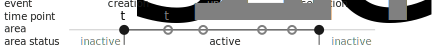
\includegraphics[width=0.9\textwidth]{graphics/development/hivent_model/area_states}
  \caption{Three event types that change Areas, resulting in two different area states}
  \label{fig:area_states}
\end{figure}

Historical changes and Areas are mutually linked, i.e.\ an Area keeps references to the changes creating, updating and deleting it and a historical change stores a set old Areas that are deleted, a set of new Areas that are created and a set of update Areas that are manipulated in the change.

% paragraph historical_changes (end)

% - - - - - - - - - - - - - - - - - - - - - - - - - - - - - - - - - - - - - - -
\paragraph{Four-Domain model} % (fold)
\label{par:four_domain_model}

Following the idea of the Three-Domain model and its extension introduced in section \ref{sub:three_domain_model}, the Hivent model is as well organized by four domains that are modeled independently from each other:

\begin{compactitem}
  \item The \emph{semantic domain} holds the Area uniquely identifiable is represented by its formal name.
  \item The \emph{spatial domain} is expressed by the territory of the Area that is visible on the map.
  \item The \emph{thematic domain} is represented by the short name of the Area.
  \item The \emph{temporal domain} is the entirety of all historical changes associated with the Area.
\end{compactitem}

The main difference between the spatial and the thematic domain is that there is no relation between the names of two Areas. While the intention is questionable, there could potentially be two Areas active at the same time with the same name. The update of the name of one Area is independent from any other Area. This is not true for the spatial domain: The territories of two Areas are highly related to each other. Geospatially, each territory has at least one neighbor and two neighbors share the same border. An update of the territory of one Area results in the update of at least one other territory.

% paragraph four_domain_model (end)

% subsection section area (end)

% ------------------------------------------------------------------------------
\subsection{Preconditions} % (fold)
\label{sub:preconditions}

\begin{quoteit}
  In the beginning God created the heavens and the Earth \\
  Now the Earth was formless and empty [...] \\
  And God said, “Let there be light” --- and there was light.
\end{quoteit}
\hfill -- Genesis 1:1, The First Book of Moses, Old Testament
\vspace{1em}


There are five axioms and two assumptions the Hivent model is based on. The theoretical foundation is the model of the Earth and its curved surface that can be projected onto a two-dimensional map using a map projection, as introduced in sections \ref{sub:geospatial_data}.

\newtheorem{invariant_surface}[assicounter]{Axiom}
\begin{invariant_surface}
\label{axm:invariant_surface}
  The Earth's surface has an invariant area size, i.e.\ it does not change over time.
\end{invariant_surface}

\vspace{-2.0em}
\newtheorem{area_on_surface}[assicounter]{Axiom}
\begin{area_on_surface}
\label{axm:area_on_surface}
  Each Area in the spatio-temporal system is located directly on the surface of the Earth.
\end{area_on_surface}

These axioms set the spatial foundation of the system: a constant dimension of the map and Areas covering the map. The basis of the temporal part of the system is content of the following axioms:

\vspace{-1.0em}
\newtheorem{initial_configuration}[assicounter]{Axiom}
\begin{initial_configuration}
\label{axm:initial_configuration}
  The spatio-temporal system is initialized at $t_0$. At this initial state, exactly one Area exists. It is denoted by $\Omega$ and is referred to as the \emph{universe} Area. It has no name and its territory covers the whole surface of the Earth.
\end{initial_configuration}

\vspace{-2.0em}
\newtheorem{historical_change}[assicounter]{Axiom}
\begin{historical_change}
\label{axm:historical_change}
  At each point $t_i \geq t_0$, multiple historical changes can be introduced.
\end{historical_change}

\vspace{-2.0em}
\newtheorem{unique_coverage}[assicounter]{Axiom}
\begin{unique_coverage}
\label{axm:unique_coverage}
  At each point $t_i \geq t_0$, each point on the surface of the Earth is covered by exactly one territory of exactly one Area.
\end{unique_coverage}

As defined in section \ref{par:area}, a historical change can create, manipulate and delete Areas on the Earth's surface. According to axiom \ref{axm:unique_coverage}, each change introduced in the system must maintain the spatial integrity on the map, i.e.\ if an Area is created on the map, the Area claiming this territory before has to secede it.

Formally, it can be said that each change consists of three sets of Areas: the old Areas $A$ that are deleted, the new Areas $B$ that are created and the Areas $C$, whose properties are updated in the change. Each $A_i \in A$ and $B_i \in B$ has a territory $A_i^T$ respectively $B_i^T$. Each $C_i \in C$ has an old territory $C_i^{OT}$ that is updated with the new territory $C_i^{NT}$. Each change introduced in the spatio-temporal system must maintain the spatial integrity of axiom \ref{axm:unique_coverage}. Therefore, the total size of the territories before the change and after the change must be the same:

\vspace{-.5em}

\[
  \left|\bigcup\limits_{i=1}^n A_i^T\right|
  +
  \left|\bigcup\limits_{i=1}^n C_i^{OT}\right|
  ~=~
  \left|\bigcup\limits_{i=1}^n C_i^{NT}\right|
  +
  \left|\bigcup\limits_{i=1}^n B_i^T\right|
\]

\vspace{.5em}

This behavior is based on to the law of conservation of energy in physics: energy in a closed system can only be transformed from one form to another, from one object to another -- but the total energy in the system is preserved at any time. In this spatio-temporal system, the total size of the territory of the Earth is preserved, but it is distributed among the active Areas in the system.

The first changes introduced in the system at $t_0$ are the creation of all bodies of water, including the oceans and lakes, denoted as $W$. Each Area $W_i \in W$ is created with their name and territory cut out of $\Omega$. The result is that after $t_0$, the map is divided into water ($W$) and land ($\Omega$). Land can at any point in time be either \emph{claimed}, i.e.\ it is currently occupied by the territory of exactly one active Area, or \emph{unclaimed}, i.e.\ belonging to $\Omega$.
% It is a subtractive data model, because each new Areas territory is cut out of $\Omega$.

\begin{figure}[ht]
  \centering
  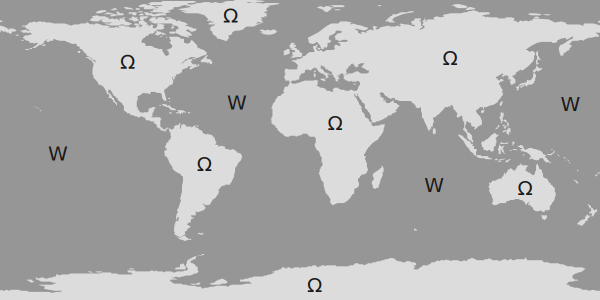
\includegraphics[width=0.6\textwidth]{graphics/development/hivent_model/init_map}
  \caption{The initial state of the world map at $t_0$}
  \label{fig:init_map}
\end{figure}

In the real world, the name of a country changes according to sudden events, e.g.\ a declaration or a governmental bill. The territory can change either because of geographical processes, e.g.\ the sea level rise influencing the coastlines, or according to a historical event, e.g.\ a treaty shifting a border between two countries. The Hivent model is based on two assumptions that simplify the model and keep the problem space clear:

\vspace{-0.0em}
\newtheorem{coastline_territory}[assicounter]{Assumption}
\begin{coastline_territory}
\label{axm:coastline_territory}
  The territory of a country stops at the coastline.
\end{coastline_territory}

\vspace{-1.5em}
\newtheorem{constant_coastlines}[assicounter]{Assumption}
\begin{constant_coastlines}
\label{axm:constant_coastlines}
  The coastlines have not changed over time.
\end{constant_coastlines}

Both assumptions are wrong. The territory of a country stretches into international water, as explained in section \ref{sub:territory_of_a_country}). Coastlines are constantly changing and so does the distribution of land and water on Earth. However, these assumptions allow the Hivent model to focus only on discrete historical changes. It is subject to future work to extend the model to account for long-term processes, e.g. the continental drifts of tectonic plates. For now, the temporal behavior of an Area in the Hivent model can be described as a \emph{static object that changes according to sudden events}.

% subsection preconditions (end)

% ------------------------------------------------------------------------------
\subsection{Hivent Operations} % (fold)
\label{sub:hivent_operations}

Respecting the preconditions, there are several different types of historical changes that transform a set of old Areas $A$ to a set of new Areas $B$ and update a set of Areas $C$. However, each possible historical change can be expressed with only one of five \emph{Hivent operations}. Four of them change the identity of at least one Area and therefore establish historical predecessor-successor-relationships. These relationships are always symmetric, i.e.\ if one old Area is replaced by one new Area, the old Area is the historical predecessor of the new Area and vice versa. The last operation changes a non-spatial property of an Area and is therefore identity-preserving.

\newpage
\begin{description}

  \item[UNI -- Unification]
  A set of old Areas unifies to one new Area. The old Areas are deleted, becoming the historical predecessors of the new Area. The territory of this new Area is the union of the territories of the old Areas. The new Area receives a new name. \\[0.25em]
  \begin{footnotesize}
    In 1922, the Russian SFSR, the Transcaucasian SFSR, the Ukrainian SSR and the Byelorussian SSR unified and formed the Union of Soviet Socialist Republics (USSR).
  \end{footnotesize}

  \item[INC -- Incorporation]
  One or more old Areas are incorporated into another Area that stays active. Its territory is enlarged by the union of the territories of the old Areas. The old Areas are historical predecessors of the Area that stays active. \\[0.25em]
  \begin{footnotesize}
    In 1990, the territory of the German Democratic Republic (East Germany) became part of the Federal Republic of Germany (West Germany). Although this event is known as the \emph{German Reunification}, it is historically an incorporation of East Germany into West Germany \cite{incorporationEastWestGermany}.
  \end{footnotesize}

  \item[SEP -- Separation]
  As the inverse of unification, one old Area is separated into multiple new Areas. Each new Area gets a part of the territory of the old Area, receives a new name, and has the old Area as its only historical predecessor. \\[0.25em]
  \begin{footnotesize}
    In 1993, the Czech and Slovak Federal Republic, commonly known as Czechoslovakia, dissolved into present-day Czech Republic and Slovak Republic, creating two new countries out of one old.
  \end{footnotesize}

  \item[SEC -- Secession]
  As the inverse of incorporation, one or more new Areas are ceded from a previously existing Area that stays active. Each new Area gets a new name, receives the previously existing Area as the only historical predecessor and a part of its territory. \\[0.25em]
  \begin{footnotesize}
    In 2008, the Republic of Kosovo declared independence from Serbia and has since then partially received international recognition. Serbia stays a country, keeping its name, but ceding a part of its territory to Kosovo.
  \end{footnotesize}

  \item[NCH -- Name Change]
  An Area changes its short name but preserves its formal name and identity. \\[0.25em]
  \begin{footnotesize}
    A recent change happened on 05.05.2016: The cabinet of Czech Republic approved that the country will now officially be called ``Czechia''. However, the formal name stays ``Czech Republic'', which preserves its identity.
  \end{footnotesize}
\end{description}

\vspace{1.5em}
\begin{table}[H]
\begin{center}
\begin{tabular}{cx{2.5cm} cx{2.5cm} cx{2.5cm} cx{2.5cm} cx{2.5cm}}

  \texttt{UNI} & \texttt{INC} & \texttt{SEP} & \texttt{SEC} & \texttt{NCH} \\
  Unification & Incorporation & Separation & Secession & Name Change \\[1em]

  
\includegraphics{graphics/development/hivent_model/operations/UNI} &
  \includegraphics{graphics/development/hivent_model/operations/INC} &
  
\includegraphics{graphics/development/hivent_model/operations/SEP} &
  \includegraphics{graphics/development/hivent_model/operations/SEC} &
  
\includegraphics{graphics/development/hivent_model/operations/NCH} \\

\end{tabular}
\caption{The five Hivent operations}
\label{tab:hivent_operations}
\end{center}
\end{table}

% subsection hivent_operations (end)

% ------------------------------------------------------------------------------
\subsection{HistoGraph} % (fold)
\label{sub:histograph}

Based on the idea of the History Graph model, introduced in section \ref{fig:history_graph_model}, the linguistically and conceptually related \emph{HistoGraph} visualizes the temporal development of countries. The edges of the graph represent an Area, the nodes a Hivent operation. The graph shows the predecessor-successor-relationships between Areas. As previously explained in section \ref{par:historical_changes}, an Area keeps references to the historical changes creating, updating and ceasing it. These changes themselves are linked to their old and new Areas. Therefore, each Area indirectly knows their successors and predecessors. The two-dimensional HistoGraph has a horizontal orientation. The x-axis refers to one point in time, the y-axis has no spatio-temporal relation. The graph uses the visualization approach of the five Hivent operations in table \ref{tab:hivent_operations}, including the following symbols:

\begin{table}[H]
\begin{center}
\begin{tabular}{c l l}

  \raisebox{3.5\height}

  \raisebox{-0.2\height}
  {
\includegraphics[width=10px]{graphics/development/hivent_model/histograph/circle_filled}}
  & Identity-changing Hivent operation
  & \texttt{UNI}, \texttt{INC}, \texttt{SEP}, \texttt{SEC} \\

  \raisebox{-0.2\height}
  {
\includegraphics[width=10px]{graphics/development/hivent_model/histograph/circle_unfilled}}
  & Identity-preserving Hivent operation
  & \texttt{NCH} \\

  \raisebox{-0.2\height}
  {
\includegraphics[width=10px]{graphics/development/hivent_model/histograph/circle_combo}}
  & A combination of both
  & e.g.\ \texttt{INC + NCH}

\end{tabular}
\label{tab:histograph_symbols}
\end{center}
\end{table}

\vspace{-2.5em}

Each uninterrupted horizontal line refers exactly to one Area. If a horizontal line leads straight through a circle, the identity of the Area is preserved in the operation. New Areas resulting from an identity-changing Hivent operation emerge from the circle with a vertical line, indicating a sudden change with a duration of zero. From this line, the new Areas branch out right-angled. The HistoGraph is created from one particular reference Area. It visualizes historically related Areas in one direction: Into the past, it recursively plots only the predecessors on the graph, but not the successors of the predecessors. Into the future, the successors of the reference Area are plotted recursively, but not their predecessors.
The behavior of the HistoGraph is shown in figure \ref{fig:example_germany} at the example of present-day Germany and its state history since the end of World War II. This history is driven by six historical events, which provide examples for all five Hivent operations. They are listed in table \ref{tab:german_history_since_1945}.

\begin{figure}[ht]
  \vspace{0.5em}
  \centering
  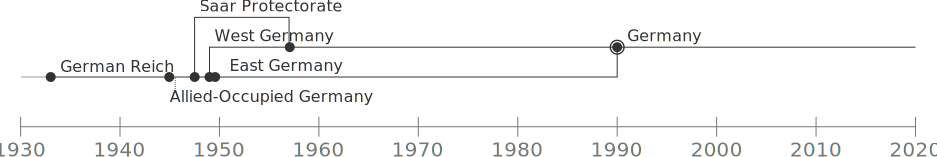
\includegraphics[width=0.9\textwidth]{graphics/development/hivent_model/histograph/example_germany}
  \caption{The concept of the HistoGraph at the example of Germany's history since 1945}
  \label{fig:example_germany}
\end{figure}


\begin{table}[ht]
\begin{center}
\begin{tabular}{l p{8.8cm} l}
  \toprule
  Hivent date & Hivent description & Hivent operations \\
  \midrule

    05.06.1945
  & \normalsize{In the Berlin Declaration the total dissolution of the Third Reich is confirmed. It separates into multiple parts, returning the territories annexed by the German Reich in World War II. The rest is controlled by the British, French, American and Soviet occupation zone.}
  & \texttt{SEP} \\[1.5em]

    16.02.1946
  & \normalsize{The Saar Protectorate is entangled from the French Zone of Occupation Germany, creating an own country.}
  & \texttt{SEC} \\[1.5em]

    28.05.1949
  & \normalsize{The Federal Republic of Germany (West Germany) is created from the British, American and French Zone of Occupation.}
  & \texttt{UNI} \\[1.5em]

    07.10.1949
  & \normalsize{The German Democratic Republic (East Germany) is created from the Soviet Zone of Occupation.}
  & \texttt{UNI} \\[1.5em]

    01.01.1957
  & \normalsize{The Saar Treaty (``Little Reunification'') joins the Saar Protectorate as the federal state ``Saarland'' in West Germany.}
  & \texttt{INC} \\[1.5em]

    03.10.1990
  & \normalsize{In the German Reunification, East joins West Germany. The Federal Republic of Germany is now called ``Germany''.}
  & \texttt{INC + NCH} \\[1.5em]

  \bottomrule
\end{tabular}
\caption{Historical events in German state history since 1945}
\label{tab:german_history_since_1945}
\end{center}
\end{table}

This example hosts a special case: In October 1949, East Germany was created from the Soviet Zone of Occupation. Both Areas have the same territory, but a different short and formal name. A \texttt{NCH} cannot be performed, because the identity is not preserved: the German Democratic Republic is a new Area. However, the change can be described by a \texttt{UNI} of only one old Area (Soviet zone), creating a new Area (East Germany). This new Area occupies exactly the same territory as the old Area and becomes the only historical successor of the old Area.

The graph plots Germany first. Since it does not have any successors, the plot expands only one way, historically backwards: East Germany and the Saar Protectorate were incorporated into Germany, so they are plotted. They emerged from the four post-war occupation zones, which are visualized in the next step. Each of the four occupation zones originated themselves from the German Reich. However, the German Reich dissolved into many more Areas, e.g.\ the Memel territory. They are not included in the graph, because they are not predecessors of any Area that is a recursive predecessor of present-day Germany.

Many problems of the graph visualization are apparent in this example: Circles may overlap if many operations happen in a short period of time -- in this case between 1945 and 1949.
The name ``West Germany'' collides with the vertical line indicating the incorporation of the Saar Protectorate, which should also be avoided.
Additionally, the names of the Areas of the four post-war occupation zones cannot be shown in the graph, due to lack of space.
One more important aspect can be seen in the foundation of West Germany in 1949: A \texttt{UNI} operation unifies three old Areas to one new Area. This could be visualized symmetrically with a straight line from the midmost incoming Area line into the circle to the outgoing Area line of the new Area. However, this would give the wrong impression that this midmost Area had the same identity as the newly created Area. In general, the circle for \texttt{UNI} and \texttt{SEP} operations with an odd number of old respectively new Areas must be displaced off the center to emphasize that the identity has changed.
All these issues are beyond the scope of this thesis and subject to future work in the field of Information Visualization.

% subsection histograph (end)

% section hivent_model (end)
%!TEX root = ../masters_thesis.tex

\section{Editing Hivent Data} % (fold)
\label{sec:editing_hivent_data}

The previous section proposed the abstract Hivent Model, a set of Hivent operations and a visualization method. However, one purpose of the HGIS developed in this thesis is to add, alter and delete historical changes. This section presents the tools and methods to edit spatio-temporal data about the evolution of Areas in the Hivent Model. Whereas the Hivent Operations are well-defined and specific, user studies have shown that they are not well understood by humans to edit Areas. This thesis therefore introduces a different set of six \emph{Edit Operations} in section \ref{sub:edit_operations}. Afterwards, section \ref{sub:edit_workflow} shows a \emph{workflow} to perform an Edit Operation step by step. The Hivent Model needs to support editing historical changes in between other historical changes. The last section \ref{sub:retrospective_updates} explains the theoretical approach to \emph{retrospecitve updates} of spatio-temporal data in the Hivent Model.


% ------------------------------------------------------------------------------
\subsection{Edit Operations} % (fold)
\label{sub:edit_operations}

The Hivent Operations are valuable, because they can describe all possible changes in the evolution of Areas in time and space. They are really well understood from the system point of view and form the basis for the Hivent Model. However, one purpose of the HGIS developed in this thesis is to provide a well understood user interface to edit historical changes to Areas.

Throughout the development process, interviews with researchers in humanities at University of Virginia were conducted to understand their mental model about the task. It turned out that the Hivent Operations are not suitable to be used for human edit purposes, because of their low-level nature. One example is that the operations do not provide a straightforward way to create a new Area on previously unclaimed land. The same is true for changing the formal name of an Area. Therefore, this thesis introduces a second set of operations: five high-level \emph{Edit Operations} describe changes to countries on the map (see table \ref{tab:edit_operations}). They have proven to be understandable in several user studies.

\vspace{0.5em}
\begin{table}[H]
\begin{center}
\begin{tabular}{m{0.75cm} m{0.8cm} m{2.4cm} m{9.1cm}}
  \raisebox{-0.35\height}
  {
\includegraphics[width=0.72cm]{graphics/development/edit_operations/CRE}} &
  \texttt{CRE} & Create &
  a new Area with a new name and territory on the map. \\

  \raisebox{-0.35\height}
  {
\includegraphics[width=0.72cm]{graphics/development/edit_operations/MRG}} &
  \texttt{MRG} & Merge &
  two or more Areas to a new Area. The name has to be set manually, the territory is automatically unified. \\

  \raisebox{-0.35\height}
  {\includegraphics[width=0.72cm]{graphics/development/edit_operations/DIS}} &
  \texttt{DIS} & Dissolve &
  one Area into two or more new Areas, manually setting their new territory and name. \\

  \raisebox{-0.35\height}
  {
\includegraphics[width=0.72cm]{graphics/development/edit_operations/CHB}} &
  \texttt{CHB} & Change Borders &
  between two neighboring Areas by defining the territory that changes sides. \\

  \raisebox{-0.35\height}
  {\includegraphics[width=0.72cm]{graphics/development/edit_operations/REN}} &
  \texttt{REN} & Rename &
  an Area and set a new formal name, short name or both. \\

  \vspace{0.35em}
  \raisebox{-0.35\height}
  {
\includegraphics[width=0.72cm]{graphics/development/edit_operations/CES}} &
  \texttt{CES} & Cease &
  an Area by deleting it from the map, leaving unclaimed land. \\

\end{tabular}
\caption{The six Edit Operations}
\label{tab:edit_operations}
\end{center}
\end{table}


% paragraph error_correction (end)

% subsection edit_operations (end)

% ------------------------------------------------------------------------------
\subsection{Edit Workflow} % (fold)
\label{sub:edit_workflow}

An Edit Operation describes an historical change that can be understood and performed by a user of the HGIS. This section shows that each Edit Operation can be internally expressed by a set of Hivent Operations. Therefore the Edit Operations are an abstraction layer in the Hivent Model between the Hivent and the Hivent Operations. To create an Edit Operation, four steps in a workflow need to be performed:

\begin{compactenum}
  \item Select the Areas that will be changed in the Edit Operation.
  \item For each new Area resulting from the Edit Operation, create a territory.
  \item For each new Area create a name.
  \item Add the Edit Operation to an Hivent to inherit the time point.
\end{compactenum}

For each Edit Operation, the requirements for the steps are different. Not all operations need all steps, because some data can be processed automatically. Table \ref{tab:editoperations_in_worklow} presents an overview about the behaviour of the Edit Operations in the first three steps. The last step is necessary for all.

\begin{table}[H]
\begin{center}
\begin{tabular}{m{0.9cm} m{4.2cm} m{4.2cm} m{3.5cm}}
  \toprule

  &
  \emph{Select old Areas} &
  \emph{Create new territories} &
  \emph{Create new names} \\

  \midrule
  \texttt{CRE} &
  -- &
  create a territory of the new country &
  create a name for the new country \\

  \midrule
  \texttt{MRG} &
  select the countries to be merged &
  \pbox{4.4cm}{--\\
  \footnotesize{territories of selected countries are automatically unified}} &
  create a name for the new country
  \\

  \midrule
  \texttt{DIS} &
  select a country to be \mbox{dissolved} &
  create a territory for each new country &
  create a name for each new country \\

  \midrule
  \texttt{CHB} &
  select two neighboring countries to change their border &
  \pbox{4.4cm}{create the new border between both countries \\
  \footnotesize{the territory for both countries will be created automatically}}  &
  -- \\

  \midrule
  \texttt{REN} &
  select a country to rename it &
  -- &
  create a new name of the country \\

  \midrule
  \texttt{CES} &
  select a country to cease it &
  -- &
  -- \\

  \bottomrule
\end{tabular}
\caption{The requirements of each step for the Edit Operations}
\label{tab:editoperations_in_worklow}
\end{center}
\end{table}

% - - - - - - - - - - - - - - - - - - - - - - - - - - - - - - - - - - - - - - -

% wording:
% UNI of "[old]"  to    "new"
% INC of "[old]"  into  "pres"
% SEP of "old"    into  "[new]"
% SEC of "[new]"  from  "pres"
% NCH of "pres"

\vspace{-1.0em}

Depending on the input of the user in the steps for an Edit Operation, there are different possibilities to express it by a set of Hivent Operations. Each Hivent Operation transforms a set of old Areas into a set of new Areas and can update the name or territory of one specific Area. All possibilities are introduced in table \ref{tab:editoperations_to_hg_operations}. Hivent Operations are combined when they happen at the same time. In the example of the German Reunification, East Germany was incorporated into West Germany which at the same time changed its short name to ``Germany'' (\texttt{INC + NCH}).

\begin{center}
\begin{longtable}{m{1.2cm} m{0.95cm} m{0.95cm} m{0.95cm} m{6.0cm} m{2.3cm}}
  \toprule

  \pbox{1.2cm}{EditOp.\\(case)} &
  \pbox{0.95cm}{old\\Areas\\[-0.8em]} &
  \pbox{0.95cm}{update\\Areas\\[-0.8em]} &
  \pbox{0.95cm}{new\\Areas\\[-0.8em]} &
  expression by Hivent Operations \protect\footnotemark &
  visualization \\
  \midrule
  \endhead

  % TODO: introduce T as territory that is used like a temporary Area with exactly that territoy

  %%% CREATE %%

  \multirow{9}{*}{\texttt{CRE} (1)} &
  \multicolumn{4}{p{10cm}}{
    Area $B_1$ is created with territory $T$. The part of $T$ that is on previously unclaimed land ($T_\Omega$) is seceded as $B_1$ from $\Omega$.
    If $T_\Omega$ is empty, then $B_1$ is initialized with an empty territory.
    The rest of $T$ covers some Areas $A_p$ partially and some Areas $A_f$ fully.
    For each $A_p$, the covered territory $T_p$ is seceded and incorporated into $B_1$.
    Each $A_f$ is completely incorporated into $B_1$.
  } &
  \multirow{9}{*}{
    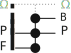
\includegraphics[width=2.5cm]{graphics/development/edit_to_hivent_operations/CRE_to_SEC+UNI}
  } \\

  &
  $n_f$ &
  $n_p$ &
  $1$ &
  \pbox{6.0cm}{
    ~\\
    \texttt{SEC} of $B_1$ from $\Omega$ \\
    \texttt{SEC} of $T_p$ from $A_p$, \texttt{INC} of $T_p$ into $B_1$ \\
    \texttt{INC} of $A_f$ into $B_1$
  } &
  \\

  %%% MERGE %%

  \midrule
  \multirow{3}{*}{\texttt{MRG} (1)} &
  \multicolumn{4}{p{10cm}}{
    Multiple Areas $A_i$ are unified to $B_1$. The new Area receives a name distinct from all the names of $A_i$.
  } &
  \multirow{3}{*}{
    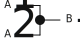
\includegraphics[width=2.5cm]{graphics/development/edit_to_hivent_operations/MRG_to_UNI}
  } \\
  &
  $n \geq 2$ &
  $0$ &
  $1$ &
  \pbox{6.0cm}{
    \texttt{UNI} of $\forall A_i$ to $B_1$
  } &
  \\

  \midrule
  \multirow{4}{*}{\texttt{MRG} (2)} &
  \multicolumn{4}{p{10cm}}{
    Multiple Areas $A_i$ are unified. The resulting Area reuses the short and formal name of one of the old Areas ($A_0$) and therefore preserves it. The remaining Areas $A_i$ are incorporated into $A_0$.
  } &
  \multirow{4}{*}{
    \includegraphics[width=2.5cm]{graphics/development/edit_to_hivent_operations/MRG_to_INC}
  } \\
  &
  $n \geq 1$ &
  $1$ &
  $1$ &
  \pbox{6.0cm}{
    \texttt{INC} of $\forall A_i$ into $A_0$
  } &
  \\

  \midrule
  \multirow{4}{*}{\texttt{MRG} (3)} &
  \multicolumn{4}{p{10cm}}{
    The same as the previous case, just that $A_0$ receives a new short name and therefore an additional name change is required.
  } &
  \multirow{4}{*}{
    \includegraphics[width=2.5cm]{graphics/development/edit_to_hivent_operations/MRG_to_INC+NCH}
  } \\
  &
  $n \geq 1$ &
  $1$ &
  $1$ &
  \pbox{6.0cm}{
    ~\\
    \texttt{INC} of $\forall A_i$ into $A_0$ \\
    \texttt{NCH} of $A_0$
  } &
  \\

  %%% DISSOLVE %%

  \midrule
  \multirow{4}{*}{\texttt{DIS} (1)} &
  \multicolumn{4}{p{10cm}}{
    Multiple Areas $B_i$ are separated from one initial Area $A_0$. Each $B_i$ receives a part of the territory of $A_0$ and a name. Each name is distinct from the name of $A_0$.
  } &
  \multirow{4}{*}{
    \includegraphics[width=2.5cm]{graphics/development/edit_to_hivent_operations/DIS_to_SEP}
  } \\
  &
  $1$ &
  $0$ &
  $n \geq 1$ &
  \pbox{6.0cm}{
    ~\\
    \texttt{SEP} of $A_1$ into $\forall B_i$
  } &
  \\

  \midrule
  \multirow{5}{*}{\texttt{DIS} (2)} &
  \multicolumn{4}{p{10cm}}{
    Multiple Areas $B_i$ are separated from one initial Area $A_0$. Each $B_i$ receives a part of the territory of $A_0$ and a name. One of the separated Areas has the same short and formal name as $A_0$, so it preserves its identity. The remaining new Areas secede from $A_0$.
  } &
  \multirow{5}{*}{
    \includegraphics[width=2.5cm]{graphics/development/edit_to_hivent_operations/DIS_to_SEC}
  } \\
  &
  $1$ &
  $1$ &
  $n \geq 1$ &
  \pbox{6.0cm}{
    ~\\
    \texttt{SEC} of $\forall B_i$ from $A_0$
  } &
  \\

  \midrule
  \multirow{4}{*}{\texttt{DIS} (3)} &
  \multicolumn{4}{p{10cm}}{
    The same as the previous case, just that $A_0$ receives a new short name and therefore an additional name change is required.
  } &
  \multirow{4}{*}{
    
\includegraphics[width=2.5cm]{graphics/development/edit_to_hivent_operations/DIS_to_SEC+NCH}
  } \\
  &
  $1$ &
  $1$ &
  $n \geq 1$ &
  \pbox{6.0cm}{
    ~\\
    \texttt{SEC} of $\forall B_i$ from $A_0$  \\
    \texttt{NCH} of $A_p$
  } &
  \\

  %%% CHANGE BORDER %%%

  \midrule
  \multirow{10}{*}{\texttt{CHB} (1)} &
  \multicolumn{4}{p{10cm}}{
    One existing Area $A_0$ is selected and its territory changes. Relative to the old territory some parts of the territory expands ($T_e$) and some withdraws ($T_w$).
    The part of $T_e$ that expands into unclaimed land ($T_\Omega: T_\Omega \in T_e$) is seceded from $\Omega$ and incorporated into $A_0$.
    The Areas $A_f$ fully covered by $T_e$ are incorporated into $A_0$,
    the Areas $A_p$ partially covered by $T_e$ secede this territory $T_p \in T_e$ to $A_0$.
    $T_w$ is be incorporated into $\Omega$, resulting in unclaimed land.
  } &
  \multirow{10}{*}{
    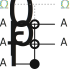
\includegraphics[width=2.5cm]{graphics/development/edit_to_hivent_operations/CHB_to_SEC+INC_omega}
  } \\
  &
  $n_f$ &
  $1+n_p$ &
  $0$ &
  \pbox{6.0cm}{
    ~\\
    \texttt{SEC} of $T_\Omega$ from $\Omega$,
    \texttt{INC} of $T_\Omega$ into $A_0$ \\
    \texttt{SEC} of $T_p$ from $A_p$,
    \texttt{INC} of $T_p$ into $B_1$ \\
    \texttt{INC} of $A_f$ into $B_1$ \\
    \texttt{SEC} of $T_w$ from $B_1$,
    \texttt{INC} of $T_w$ into $\Omega$
  } &
  \\

  \midrule
  \multirow{7}{*}{\texttt{CHB} (2)} &
  \multicolumn{4}{p{10cm}}{
    Two existing Areas $A_1$ and $A_2$ are selected and their common border changes. This results in a symmetrical change of territories, made up by two sets of territories: $T_2$ that previously belonged to $A_1$ and is now part of $A_2$ and $T_1$ for which the opposite is true. $T_2$ is seceded by $A_1$ and incorporated into $A_2$, the opposite happenes to $T_1$.
  } &
  \multirow{7}{*}{
    \includegraphics[width=2.5cm]{graphics/development/edit_to_hivent_operations/CHB_to_SEC+INC}
  } \\
  &
  $0$ &
  $2$ &
  $0$ &
  \pbox{6.0cm}{
    ~\\
    \texttt{SEC} of $T_2$ from $A_1$,
    \texttt{INC} of $T_2$ into $A_2$ \\
    \texttt{SEC} of $T_1$ from $A_2$,
    \texttt{INC} of $T_1$ into $A_1$
  } &
  \\

  %%% RENAME %%%

  \midrule
  \multirow{3}{*}{\texttt{REN} (1)} &
  \multicolumn{4}{p{10cm}}{
    One Area $A_1$ is selected and both its short and formal name is changed. Therefore, a new Area $B_1$ is created as a direct successor of $A_1$. This is a special case of a unification with only one Area.
  } &
  \multirow{3}{*}{
    \includegraphics[width=2.5cm]{graphics/development/edit_to_hivent_operations/REN_to_UNI}
  } \\
  &
  $1$ &
  $0$ &
  $1$ &
  \pbox{6.0cm}{
    \texttt{UNI} of $A_1$ to $B_1$
  } &
  \\

  \midrule
  \multirow{3}{*}{\texttt{REN} (2)} &
  \multicolumn{4}{p{10cm}}{
    One Area $A_1$ is selected and receives a new short name, but the formal name and therefore the identity is preserved. $A_1$ is updated.
  } &
  \multirow{3}{*}{
    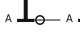
\includegraphics[width=2.5cm]{graphics/development/edit_to_hivent_operations/REN_to_NCH}
  } \\
  &
  $0$ &
  $1$ &
  $0$ &
  \pbox{6.0cm}{
    \texttt{NCH} of $A_1$
  } &
  \\

  %%% CEASE %%%

  \midrule
  \multirow{2}{*}{\texttt{CES} (1)} &
  \multicolumn{4}{p{10cm}}{
    One Area $A_1$ is selected and ceases by incorporating into the universe.
  } &
  \multirow{2}{*}{
    \includegraphics[width=2.5cm]{graphics/development/edit_to_hivent_operations/CES_to_INC}
  } \\
  &
  $1$ &
  $0$ &
  $0$ &
  \pbox{6.0cm}{
    \texttt{INC} of $A_1$ into $\Omega$
  } &
  \\

  \bottomrule
\caption{Translation from Edit Operations to Hivent Operations}
\end{longtable}
\label{tab:editoperations_to_hg_operations}
\end{center}
\footnotetext{multiple Hivent Operations in one row happen exactly at the same time point, so they are combined}


% subsection edit_workflow (end)

% ------------------------------------------------------------------------------
\subsection{Retrospective Updates} % (fold)
\label{sub:retrospective_updates}

A straighforward use case of the Hivent Model is to change the current state of the system with a new Edit Operation into the future. Givent the initial start point $t_0$, a current time point $t_{now} > t_0$ and a set of consecutively added Hivent Operations at $t_i \in [t_0 .. t_{now}[$. The accumulation of all changes make up the current state of the system at $t_{now}$. To change this current state, a new Hivent Operation can be inserted at $t_{now}$ into the future as a \emph{forward operation}. This state is valid until the next change is inserted.

For the purpose of historical research this use case alone is not sufficient, because the current state $t_{now}$ of the map is known to large degree. The problem is to edit states in the past. For this purpose the concept of a \emph{backward operation} comes into play: A Hivent Operation is inserted at time point $t_i$, but into the past: $ t_0 < t_i < t_{now}$. As an example: Given the initial state 10.06.2016 with present-day Germany created on 03.10.1990 on the map. The user wants to enter the German Reunification. The HGIS must support separating Germany into East and West, but indicating that this was the state \emph{before} 1990 and the original state was \emph{after} this date. This is complicated, because the conceptual, data and computational model have to adapt to this requirement.

The Hivent Operations themselves allow to be executed the other way, because each of them has an inverse operation: A \texttt{UNI} can be inverted with a \texttt{SEP} and a \texttt{INC} with a \texttt{SEC} operation. \texttt{NCH} can be inverted with itself by swapping the old and new name.

% - - - - - - - - - - - - - - - - - - - - - - - - - - - - - - - - - - - - - - -
\paragraph{Consistency} % (fold)
\label{par:consistency}

Each Hivent Operation that is not entered as a \emph{forward operation} to the end of the timeline must maintain the semantic, spatial and thematic integrity of the data, i.e. the changes to Areas, their territories and names must still work. All possible conflicts with consecutive Hivent Operations have to be resolved. The simple example in figure \ref{fig:update_conflict_example} shows the problem: Given time point $t_1$ with two Areas $A$ and $B$ and an \texttt{UNI} Hivent Operation at $t_2$ unifying $A$ and $B$ to $C$. If in retrospective a new Hivent Operation is inserted at $t_r: t_1 < t_r < t_2$ that cedes a part of of $A$ to a new Area $X$, the operation at $t_2$ is not consistent anymore, because the old territory of $A$ is not the same. It is not simple to say how the remaining territory $?$ should be treated.

\begin{figure}[H]
  \vspace{1em}
  \centering
  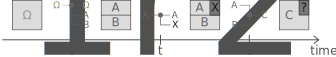
\includegraphics[width=0.8\textwidth]{graphics/development/update_conflict/example}
  \caption{Example for a simple conflict due to a retrospective update}
  \label{fig:update_conflict_example}
\end{figure}

% paragraph consistency (end)

% - - - - - - - - - - - - - - - - - - - - - - - - - - - - - - - - - - - - - - -
\paragraph{Conflicts} % (fold)
\label{par:conflicts}

The way the Hivent Model works is comparable to a version control system like \emph{Git}
\footnote{
  \emph{Git},
  --everything-is-local,
  \url{https://git-scm.com/},
  last access: 29.05.2016
}
Just like in Git, there are different kinds of conflicts that can occur on retrospective updates. In this model, they are classified regarding their resolvability:

\begin{compactenum}
  \item[A)] The conflict can be resolved \emph{\textbf{a}utomatically} without the interference of the user.
  \item[S)] The conflict requires the user to choose between two alternatives (\emph{\textbf{s}emi-automatic} resolution).
  \item[M)] The conflict is complex and the user needs to resolve it \emph{\textbf{m}anually}.
\end{compactenum}

The remaining part of this section examines all possible cases of conflicts and their resolveability. Each inserted Hivent Operation transforms a set of old Areas $A = [A_i]$ to a set of new Areas $B = [B_i]$ or updates an update Area $A_0$ or both. Each consecutive Hivent Operation that manipulates $A_0, A_i \in A$ or $B_i \in B$ has to be checked regarding three aspects of integrity:

\begin{compactenum}
  \item semantic: Does $A_0$ and $\forall A_i \in A$ still exist? If not, can it easily be replaced by another Area?
  \item spatial: Is the territory of $A_0$ and $\forall A_i \in A$ still the same? If not, can it easily by updated?
  \item thematic: Is the name of $A_0$ and $\forall A_i \in A$ still the same? If not, can it easily be updated?
\end{compactenum}

All cases can be broken down to the following scenario. Given an initial state at $t_1$ with three spatial entities on the map ($A_1, A_2, A_3$) and an Hivent Operation at $t_2$ manipulating this set of Areas with one of the five possible operations. This is operation is consistent and is called the original Hivent Operation ($H_o$). Now, a retrospective update $H_r$ with one of the five Hivent Operations manipulating the same set of Areas is inserted at $t_r: t_1 < t_r < t_2$. What happens regarding the semantic, spatial and thematic integrity of $H_o$? There are 25 possible cases, because there are 5 different $H_o$ and five different $H_r$ operations.

% paragraph conflicts (end)

% - - - - - - - - - - - - - - - - - - - - - - - - - - - - - - - - - - - - - - -
\paragraph{Retrospective Unification} % (fold)
\label{par:retrospective_unification}
\texttt{UNI}

% paragraph retrospective_unification (end)

% - - - - - - - - - - - - - - - - - - - - - - - - - - - - - - - - - - - - - - -
\paragraph{Retrospective Separation} % (fold)
\label{par:retrospective_separation}
\texttt{SEP}

% paragraph retrospective_separation (end)

% - - - - - - - - - - - - - - - - - - - - - - - - - - - - - - - - - - - - - - -
\paragraph{Retrospective Incorporation} % (fold)
\label{par:retrospective_incorporation}
\texttt{INC}

% paragraph retrospective_incorporation (end)

% - - - - - - - - - - - - - - - - - - - - - - - - - - - - - - - - - - - - - - -
\paragraph{Retrospective Secession} % (fold)
\label{par:retrospective_secession}
\texttt{SEC}

% paragraph retrospective_secession (end)

% - - - - - - - - - - - - - - - - - - - - - - - - - - - - - - - - - - - - - - -
\paragraph{Retrospective Name Change} % (fold)
\label{par:retrospective_name_change}
\texttt{NCH}

trallala und hoppsassa

% paragraph retrospective_name_change (end)

\vspace{1em}
The final result is visualized in the $5 \times 5$ matrix in figure \ref{tab:conflicts_retrospective_updates}.

\begin{table}[ht]
\begin{center}
\begin{tabular}{p{0.1cm} p{0.1cm} p{0.3cm} cx{2.0cm} cx{2.0cm} cx{2.0cm} cx{2.0cm} cx{2.0cm} cx{2.0cm}}
  \toprule
  & & & & \multicolumn{5}{c}{original Hivent Operation $H_o$} \\
  & & & & \texttt{UNI} & \texttt{SEP} & \texttt{INC} & \texttt{SEC} & \texttt{NCH} \\
  \midrule
    \multirow{5}{*}{\rot{retrospective}}
  & \multirow{5}{*}{\rot{operation $H_r$}}
    & & \texttt{UNI} & A & \textbf{M} & A & A & A \\
  & & & \texttt{SEP} & S(A$|$A) & S(A$|$A) & \textbf{M} & S(A$|$\textbf{M}) & A \\
  & & & \texttt{INC} & A & \textbf{M} & A & A & X \\
  & & & \texttt{SEC} & S(A$|$A) & S(A$|$A) & S(A$|$A) & S(A$|$A) & X \\
  & & & \texttt{NCH} & A & A & X & X & A \\
  \bottomrule
\end{tabular}
\caption{All possible conflicts on retrospective updates regarding their resolvability}
\small{X = no conflict, A = automatic, S = semi-automatic, \textbf{M} = manual resolution \\[-0.1em]
For semi-automatic resolution, the resolveability of the two options is stated like S(\nth{1}$|$\nth{2})}
\label{tab:conflicts_retrospective_updates}
\end{center}
\end{table}

% - - - - - - - - - - - - - - - - - - - - - - - - - - - - - - - - - - - - - - -
\paragraph{Error correction} % (fold)
\label{par:error_correction}

Correcting wrong information in an event-based system is important to understand: Given time point $t_y$ and an Area $A$ with the name $X$. If $X$ happens to be wrong, it means that the historical change at time point $t_x: t_x < t_y$ that created the name $X$ into Area $A$ is erroneous and has be corrected. Correcting a state means correcting the event that created this state.

% subsection retrospective_updates (end)

% section editing_hivent_data (end)
%!TEX root = ../masters_thesis.tex

\section{User Interface Design Process} % (fold)
\label{sec:user_interface_design_process}

The Hivent Model presented in the previous section serves as the data model for HistoGlobe, the application in which the work of this thesis is implemented. Developing the system bottom-up from the data model to the interface might not lead to usable system. Human Centered Design promotes a top-down process from the user via the interface into the core of the application. This section illustrates the iterative design process for this thesis seen in figure \ref{fig:hcd}. The two main use cases for HistoGlobe that are focused in this thesis are:

\begin{compactenum}
  \item \textbf{Understanding} the history of countries.
  \item \textbf{Editing} the spatio-temporal evolution of countries with historical changes.
\end{compactenum}

For both use cases a visualization and interaction was designed. The interviews with humanity researchers confirmed that the combination of a map and a timeline are a very appropriate and intuitive way to interactively visualize the history of countries. Thefore, the main concept of HistoGlobe introduced in section \ref{sec:histoglobe} does not need to be changed. However, two necessary extension modules have emerged: The \emph{HistoGraph} introduced in section \ref{sub:histograph} visualizes the history of countries on a graph. Next to the normal browsing mode, the \emph{Edit Mode} is proposed in section \ref{sub:edit_mode}. It uses the six Edit Operations to introduce historical changes to the current state on the map. The gradual process from the inital idea to the final user interface implemented in HistoGlobe is illustrated in the last section-

The user interface of HistoGlobe has two modi: The browsing mode to view the evolution of countries on a map with a timeline and the \emph{Edit Mode} to introduce historical changes to Areas. This mode is proposed in this section. The Human Centered Design process produced an interface that allows to intuitively edit Hivents, Areas and historical changes directly in HistoGlobe, without the need to write data into tables or forms.

The previous sections introduced the concepts of the HistoGraph and the Edit Mode. This section illustrates the Human Centered Design process integrating both concepts into the existing user interface of HistoGlobe. In each phase, interviews with students and employees of Scholar's Lab at University of Virginia were conducted to determine what works well and what has to be improved.

% - - - - - - - - - - - - - - - - - - - - - - - - - - - - - - - - - - - - - - -
\subsection{Initial interviews} % (fold)
\label{sub:initial_interviews}

The first phase, four researchers were asked about their opinions on the idea of HistoGlobe, potential use cases and the concept of the Edit Mode. The idea proved popular, especially for students and teachers in school, historically interested people in general and also for scholars in digital humanities. All researchers agreed that the key to successful Edit Mode is usability, because editing data in time and space is a challenging task. A main concern is uncertainty in historical research: Almost all sorts of information -- temporal, spatial and attribute -- are potentially uncertain. A good user interface for researchers therefore has to support uploading historical sources and indicating uncertainty. The Edit Operations from section \ref{sub:edit_operations} resulted from the initial interviews.

% subsection initial_interviews (end)


% - - - - - - - - - - - - - - - - - - - - - - - - - - - - - - - - - - - - - - -
\subsection{Paper Prototype} % (fold)
\label{sub:paper_prototype}

From the results of the inital interview, the first interface concept for the Edit Mode was developed and transformed into a paper prototype. It is an interface out of paper that is very fast to create and allows to identify flaws in the concept early in the design process. In this process, two paper prototype iterations were created. Both iteration took about three full work days: one day to create the conceptualize and create prototype, half a day to conduct the study with three people, and one and a half days to analyze the results and rethink the concept.

\begin{figure}[H]
\centering
\begin{subfigure}{.5\textwidth}
  \centering
  \includegraphics[width=225px]{graphics/development/design_process/paper_prototype_1.png}
\end{subfigure}%
\begin{subfigure}{.5\textwidth}
  \centering
  \includegraphics[width=225px]{graphics/development/design_process/paper_prototype_2.png}
\end{subfigure}
\caption{The two iteration of the paper prototype for the Edit Mode}
\label{fig:paper_prototypes}
\end{figure}

The interface consists of a map of Europe, a timeline centered at 1975 and the buttons with a set of dialogs for the for the Edit Mode. Both prototypes were evaluated with three test subjects that had to solve four tasks covering different use cases and operations:
\begin{compactenum}
  \item 1300: Rename incorrectly spelled name of Switzerland on the map (\emph{correction})
  \item 1990: Unite East and West Germany (\emph{forward change})
  \item 1993: Separate the Soviet Union into Russia, Estonia, Latvia, etc. (\emph{forward change})
  \item 1944: Change the border between Finland and the Soviet Union before 1944 (\emph{backward change})
\end{compactenum}

Most parts of the interface concept were understood and all subjects could solve the first three tasks. However, there were also problems:

\begin{compactenum}
  \item There difference between Hivents, the history of a country and an historical change was unclear.
  \item The border drawing dialoge was imagined to be very complex.
  \item The backward change was not understood
  \item Correcting the name Switzerland by changing the event that created it in 1300 caused confusion.
\end{compactenum}

The main finding of this step was that depending on the task, there is both an Hivent-based and an Area-based mental model of the task. This became apparent in the German Reunification Hivent: Some users started the unification operation first, and added West and East Germany afterwards -- and some selected first West Germany, then initiated a unification operation and then added East Germany. From that finding arose that the interface has to support both an Hivent-based and an Area-based approach to introduce historical changes and correct information on the map.

% subsection paper_prototype (end)

% - - - - - - - - - - - - - - - - - - - - - - - - - - - - - - - - - - - - - - -
\subsection{Mockup Prototype} % (fold)
\label{sub:mockup_prototype}

The main part of the design process was spent on the mockup prototypes. Their purpose is to rapidly develop an interface workflow that is understandable by the users. The prototypes were created in \emph{LibreOffice Impress}, an open-source slide-based presentation tool. The interface is simulated on slides: the map is a background image, the timeline, the set of buttons and dialogs for the Edit Mode and HistoGraph are modelled with geometric elements: lines, circles and rectangles. Interactivity is simulated by linking a click on an element to a different slide that shows the effect of the operation. This allows to model sudden changes in the interface.

\begin{figure}[ht]
  \centering
  \begin{subfigure}[b]{.5\textwidth}
    \centering
    \includegraphics[width=180px]{graphics/development/design_process/mockup_prototype_1.png}
  \end{subfigure}%
  \begin{subfigure}[b]{.5\textwidth}
    \centering
    \includegraphics[width=180px]{graphics/development/design_process/mockup_prototype_3.png}
  \end{subfigure} \\[0.8em]

  % \begin{subfigure}[b]{1.0\textwidth}
  %   \centering
  %   \includegraphics[width=325px]{graphics/development/design_process/mockup_prototype_3.png}
  % \end{subfigure}
  \caption{Two iteration stages of the mockup prototype for the Edit Mode}
  \label{fig:mockup_prototypes}
\end{figure}

Creating the mockup prototype took longer than a paper prototype, but would have still been much faster than actually implementing an interactive Web-based interface. Each prototype iteration was tested with multiple subjects and similar tasks as for the paper prototype. From one test to the next one changes to the interfaces were made. Some interesting quotes from the users were:

\begin{quoteit}
  \begin{tabular}{l r}
    ``this was much easier than I thought'' ~~~~~~~~ &
    ``there is a training session needed'' \\[0.5em]
    ``the interface is very clear &
    ``the logic makes sense, \\
    and graphically pleasing'' &
    it is just very complex'' \\[0.5em]
    ``it's looking good'' &
    ``a nice tutorial and a good \\
    & documentation are necessary'' \\
  \end{tabular}
\end{quoteit}

The main evolution was from a separate dialogue window for the Edit Operation workflow to an intergrated workflow window in the title bar. Also the HistoGraph was introduced to visualize the historical change at while editing it. A lot of smaller design issues, e.g. position of buttons, font sizes or color schemes were identified and fixed. But also conceptual issues arose.

Especially the problem to initiate a backward change (see section \ref{fig:backward_change}) proved to be very difficult. Two design solutions were developed: First, instead of initializing a change in 1990 to separate Germany into East and West, the user can introduce two creation events for the two German states in May and October 1949. The interface needs to provide a visual clue that after creating West Germany, this Area can only be active until 1990, because then another Area, present-day Germany, uses its territory (see figure \ref{sfig:backward_change_1}). The change from West Germany to Germany will be created automatically. The second approach is to introduce a button that flippes an Edit Operation that has just been created (see figure \ref{sfig:backward_change_2}) -- in this case the \texttt{DIS} operation introduced to secede East Germany from Germany will be flipped into a \texttt{UNI} operation to incorporate East Germany into Germany. This approach makes use of the fact that each Edit Operation and has an inverse, as explained in section \ref{par:inverse_operations}.
However, this flipping requires the introduction of additional creation events: West and East Germany were introduced in the change, but only the event that ceases both of them (\texttt{INC} of West Germany into East Germany). They also need a creation event, otherwise they would be active backwards all the way to $t_0$, the initial state of the system.

\begin{figure}[ht]
\centering
\begin{subfigure}[b]{.5\textwidth}
  \centering
  \includegraphics[width=200px]{graphics/development/design_process/backward_change_1.png}
  \caption{Visual clue: predefined and of Area}
  \label{sfig:backward_change_1}
\end{subfigure}%
\begin{subfigure}[b]{.5\textwidth}
  \centering
  \includegraphics[width=200px]{graphics/development/design_process/backward_change_2.png}
  \caption{Create backward change by flipping Edit Operation}
  \label{sfig:backward_change_2}
\end{subfigure}
\caption{Two approaches for editing changes backwards}
\label{fig:backward_change}
\end{figure}

The prototype was very valuable for the development process. In a total of two weeks, an interface concept and workflow was designed that proved to be understandable by the users.


% subsection mockup_prototype (end)

% - - - - - - - - - - - - - - - - - - - - - - - - - - - - - - - - - - - - - - -
\subsection{Web-based prototype} % (fold)
\label{sub:web_based_prototype}

The main advantage of the design process is that it prevents major redesigns of the final Web-based prototype. After three months of implementation of the final system, the interface looks very similar to the last version of the mockup prototype. The original main elements of the interface are the map, the timeline with the Now Marker indicating the current date of the visualization and the control buttons for zooming the map and the timeline. They are preserved and extended by new interface elements for the Edit Mode. Their interaction and behavior are introduced in this section at the example of the fictional secession of Scotland from the United Kingdom in 2018. The HistoGraph was not implemented, because of the conceptual problems mentioned in section \ref{sub:histograph} that have to be solved first.

\newpage
\begin{minipage}[t]{0.47\textwidth}

  \begin{figure}[H]
    \centering
    \includegraphics[width=1.0\textwidth]{graphics/development/final_interface/1_init.png}
    \caption{Initial state of the normal mode}
    \label{fig:final_1_init}
  \end{figure}

  The initial state of the user interface. Additional to the original elements, there is an edit button on the upper right corner. Clicking it enters the Edit Mode of the system.

\end{minipage}    % N.B. the % is very important
\hspace{1.5em}    % N.B. this must go in this line, no blank lines !!!
\begin{minipage}[t]{0.47\textwidth}

  \begin{figure}[H]
    \centering
    \includegraphics[width=1.0\textwidth]{graphics/development/final_interface/2_edit_mode.png}
    \caption{Initial state of the Edit Mode}
    \label{fig:final_2_edit_mode}
  \end{figure}

  In the Edit Mode, a title bar and six buttons for the Edit Operations are   revealed. Clicking a button starts the operation workflow introduced in section \ref{par:workflow}.

\end{minipage}

\vspace{1em}
\begin{minipage}[t]{0.47\textwidth}

  \begin{figure}[H]
    \centering
    \includegraphics[width=1.0\textwidth]{graphics/development/final_interface/3_select_old_areas.png}
    \caption{Step 1) \texttt{SELECT\_OLD\_AREAS}}
    \label{fig:final_3_select_old_areas}
  \end{figure}

  A \emph{Workflow Window} is guiding the user through the process of completing the historical change. It shows all the steps necessary for this Edit Operation. In the case of \texttt{DIS}, the user has to select the country to be dissolved by clicking it on the map. After the step is completed, clicking the next button in the workflow window procceeds to the next step. At each point in the workflow, clicking the back button reverts the previous action.

\end{minipage}    % N.B. the % is very important
\hspace{1.5em}    % N.B. this must go in this line, no blank lines !!!
\begin{minipage}[t]{0.47\textwidth}

  \begin{figure}[H]
    \centering
    \includegraphics[width=1.0\textwidth]{graphics/development/final_interface/4_set_new_territories.png}
    \caption{step 2) \texttt{SET\_NEW\_TERRITORIES}}
    \label{fig:final_4_set_new_territories}
  \end{figure}

  In the second step, the user has to create the territory for each new Area that shall be created. Therefore, the \emph{New Territory Tool} provides the functionality to create, manipulate and delete polylines by clicking and moving it directly on the map. The polypolygon drawn by the user is intersected with the old territory to create the territory of the new Area. After one new territory is created sucessfully, the second one can be taken from the remaining old territory by selecting it from the map. As soon as the whole old territory is distributed among the new Areas, the workflow proceeds to the next step.

\end{minipage}

\vspace{1em}
\begin{minipage}[t]{0.47\textwidth}

  \begin{figure}[H]
    \centering
    \includegraphics[width=1.0\textwidth]{graphics/development/final_interface/5_set_new_name.png}
    \caption{Step 3) \texttt{SET\_NEW\_NAMES}}
    \label{fig:final_5_set_new_name}
  \end{figure}

  In the next step, for each Area that has been created in the step before, a name has to be defined. The \emph{New Name Tool} is a draggable input form with two lines, the upper one for the short name, the lower one for the formal name, the identity of the Area. Via instant search, the user can select existing country names from the database to be put in the New Name Tool. When clicking the confirm button, the short name is put directly on the map.

\end{minipage}    % N.B. the % is very important
\hspace{1.5em}    % N.B. this must go in this line, no blank lines !!!
\begin{minipage}[t]{0.47\textwidth}

  \begin{figure}[H]
    \centering
    \includegraphics[width=1.0\textwidth]{graphics/development/final_interface/6_add_change_to_hivent_1.png}
    \caption{Step 4) \texttt{ADD\_CHANGE}}
    \label{fig:final_6_add_change_to_hivent_1}
  \end{figure}

  When all names are set, the Edit Operation is complete. In the last step of the workflow, it has to be added to an Hivent. The \emph{New Hivent Box} offers two possibilities: the user can search for an existing Hivent and add the historical change to it, or create a new one.

\end{minipage}

\vspace{1em}
\begin{minipage}[t]{0.47\textwidth}

  \begin{figure}[H]
    \centering
    \includegraphics[width=1.0\textwidth]{graphics/development/final_interface/7_add_change_to_hivent_2.png}
    \caption{Step 4) \texttt{ADD\_CHANGE}}
    \label{fig:final_7_add_change_to_hivent_2}
  \end{figure}

  The new Hivent created for that change is the ``Scottish Independence'' on 01.01.2018 with a description of the Hivent and possibly a location and a link to a wikipedia article. In the last line, the historical change ``Secession of Scotland from the United Kingdom'' is noted. Clicking the confirm button finalizes the workflow.

\end{minipage}    % N.B. the % is very important
\hspace{1.5em}    % N.B. this must go in this line, no blank lines !!!
\begin{minipage}[t]{0.47\textwidth}

  \begin{figure}[H]
    \centering
    \includegraphics[width=1.0\textwidth]{graphics/development/final_interface/8_final_state.png}
    \caption{The final state with Scotland}
    \label{fig:final_8_final_state}
  \end{figure}

  Clicking the edit button again leaves the Edit mode back to the normal view. Scotland and the United Kingdom are both visible on the map after 2018. When moving the timeline before 2018, Scotland is still part of the UK.

\end{minipage}

% subsection web_based_prototype (end)

% section user_interface_design_process (end)
%!TEX root = ../masters_thesis.tex

\section{Application} % (fold)
\label{sec:application}

HistoGlobe is a Web-based Historical Geographic Information System. The Data model and the conceptual model of the user interface were introduced in the first sections of this chapter. This section introduces the underlying database model, a specific implementation of the data model, and the computational model that translates between the conceptual model and the database model. The first part provides an overview about the architecture of the system in section \ref{sub:system_architecture}.
% ... bla bla bla, the rest comes last
% problems
% - support uncertainty

% ------------------------------------------------------------------------------
\subsection{System Architecture} % (fold)
\label{sub:system_architecture}

HistoGlobe uses a classical client-server architecture of a Web-based information system. The user opens the application and interacts with it through the user interface in a Web browser, the \emph{client} side of the system. The Web \emph{server} is a remote computer that hosts the database and the middleware. The user interacts with the interface and the client-side application sends a request to the Web server for new data. The middleware checks the request and queries the necessary data from the database. It transforms the data and sends it back to the client. The interface shows the new information.

\begin{figure}[H]
  \vspace{1em}
  \centering
  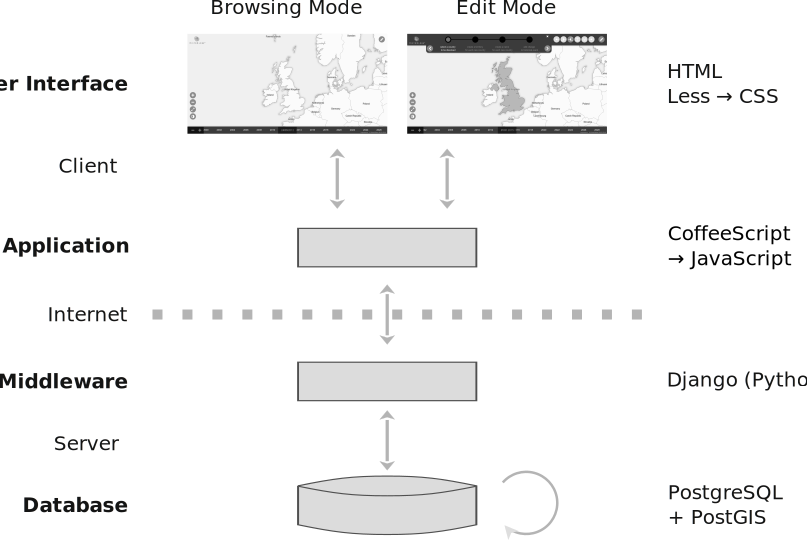
\includegraphics[width=0.7\textwidth]{graphics/development/system_architecture}
  \caption{The system architecture of HistoGlobe}
  \label{fig:system_architecture}
\end{figure}

This clear separation between the data, the application and the user interaction in this chapter and in the system follows directly from the \emph{model-view-controller} pattern: One part can be changed independently from the others parts: if the 2D map is replaced by a 3D globe, only the view changes, but the middleware and the database can stay untouched. Likewise, the implementation of a new database technology has no consequences to the view.

% subsection system_architecture (end)

% ------------------------------------------------------------------------------
\subsection{Hivent Database Model} % (fold)
\label{sub:database_model}

The underlying Hivent Model is implemented in the spatio-temporal \emph{Hivent Database Model}. HistoGlobe uses \emph{Django}, a free and open-source web framework
\footnote{
  \emph{Django},
  The Web framework for perfectionists with deadlines,
  URL: \url{https://www.djangoproject.com/},
  last access: 27.05.2016
},
combined with \emph{PostgreSQL}
\footnote{
  \emph{PostgreSQL:},
  The world's most advanced open source database,
  URL: \url{http://www.postgresql.org/},
  last access: 31.10.2015
}
, one of the most popular Object-Relational Database Management Systems introduced in section \ref{sub:object_relational_database_management_systems}, on the server-side of the system. This allows HistoGlobe to take advantage of object-oriented concepts in a stable and fast relational database. Since the database is using a lot of geospatial data, \emph{PostGIS} is used as a spatial database extension for PostgreSQL
\footnote{
  \emph{PostGIS},
  Spatial and Geographic Objects for PostgreSQL,
  URL: \url{http://postgis.net/},
  last access: 27.05.2016
}.

With these tools at hand, the database model shown in figure \ref{fig:database_model_er} was developed. It is the final result of a highly iterative process that underwent many improvements and adpations to new requirements introduced in the Human Centered Design process. The model is structured in two parts covereing four different domains of the spatio-temporal model: The lower part describes the semantic, spatial and thematic domain of Areas and the upper part represents the temporal domain of Hivents that introduces changes to the Areas.

\begin{figure}[ht]
  \centering
  \includegraphics[width=0.8\textwidth]{graphics/development/database_model/er_model}
  \caption{The Hivent Database Model}
  \small{Each entity additionally has an \texttt{id} attribute, which is omitted for simplification purposes.}
  \label{fig:database_model_er}
\end{figure}

% - - - - - - - - - - - - - - - - - - - - - - - - - - - - - - - - - - - - - - -
\paragraph{Semantic, Spatial and Thematic Domain} % (fold)
\label{par:semantic_spatial_and_thematic_domain}

In the Hivent Model, the entity visible on the map is an Area with a name and a territory, as introduced in section \ref{sec:hivent_model}. In the database model, they are represented by three entities:

\begin{enumerate}
  \item \texttt{Area}: semantic domain defining one identical Area with potentially changing name and territory. The \texttt{universe} attribute is true for $\Omega$, for the other Areas it is false.
  \item \texttt{AreaTerritory}: spatial domain. A polypolygon describes the \texttt{geometry} of the territory and a \texttt{representative\_point} the position of the name label on the map.
  \item \texttt{AreaName}: thematic domain. It is defined by a \texttt{short\_name} and a \texttt{formal\_name}.
\end{enumerate}

% paragraph semantic_spatial_and_thematic_domain (end)

% - - - - - - - - - - - - - - - - - - - - - - - - - - - - - - - - - - - - - - -
\paragraph{Temporal Domain} % (fold)
\label{par:temporal_domain}

The main idea of the model is that the Areas can change over time. These changes are introduced by \texttt{Hivents}, the main entitity of the eponymic model with five attributes: The \texttt{name} and a textual \texttt{description} of the Hivent, the point in time the Hvent happend (\texttt{date}), the Hivent \texttt{location} as a simple string and a \texttt{link} (URL) to the related article, serving as a historical source. Each Hivent can introduce a set of \texttt{EditOperation}s introduced and understood by the user. They consist themselves of a set of low-level \texttt{HiventOperation}s). They replace a set of \texttt{OldArea}s with a set of \texttt{NewArea}s and might update the name or the territory of one specific \texttt{UpdateArea}.

% paragraph temporal_domain (end)

% - - - - - - - - - - - - - - - - - - - - - - - - - - - - - - - - - - - - - - -
\paragraph{Example} % (fold)
\label{par:example}

Figure \ref{fig:database_example_reunification} shows the Hivent Database Model at the example of the German Reunification on 3. October 1990. Before 1990, there were the Areas \texttt{GDR} (``German Democratic Republic'', East Germany) and \texttt{FRG} (``Federal Republic of Germany'', West Germany). A user introduced a Merge operation (\texttt{MRG}) in the Edit Mode between \texttt{FRG} and \texttt{GDR}. The new Area received the short name ``Germany'' and the same formal name ``Federal Republic of Germany'' as previous West Germany. Internally, the Edit Mode translates this to an \texttt{INC} of \texttt{GBDR} into \texttt{FRG} and a subsequent \texttt{NCH} of the \texttt{FRG}. One Area ceases, one Area is updated twice and no new Area is created.

\begin{figure}[ht]
  \vspace{1em}
  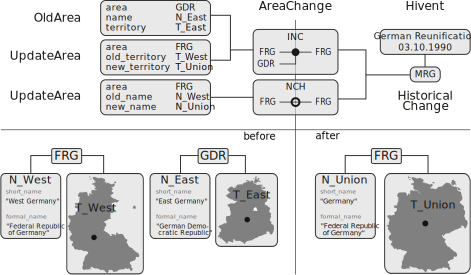
\includegraphics[width=0.9\textwidth]{graphics/development/database_model/example_reunification}
  \caption{Visualization of the German Reunification in the Hivent Database Model}
  \label{fig:database_example_reunification}
\end{figure}


% paragraph example (end)

% - - - - - - - - - - - - - - - - - - - - - - - - - - - - - - - - - - - - - - -
\paragraph{Initial Dataset} % (fold)
\label{par:initial_dataset}

Section \ref{sub:data_sources} explained the lack of data about historical countries. It is out of the scope of this thesis to create a large testing dataset with the historical countries in the world. The inital dataset consists of the following countries, their names and borders: the 193 UN members and 2 observer states (created by \texttt{CRE} operation) and seven countries with limited international recognition: Kosovo, Transnistria, South Ossetia, Abkhazia, Nagorno-Karabakh, Somaliland and Sahrawi Arab Democratic Republic, see section \ref{par:un_non_members_with_limited_recognition}) (created by \texttt{DIS} operations from their homeland on the day of their declaration of independence).

% paragraph initial_dataset (end)

% - - - - - - - - - - - - - - - - - - - - - - - - - - - - - - - - - - - - - - -
\paragraph{Middleware} % (fold)
\label{par:middleware}

The Django web framework provides \emph{view} classes as the middleware that receives requests from the client, processes them, queries the necessary data from the database and returns an \texttt{HttpResponse} back to the client. In the naive implementation of the system, the middleware provides only two views for the two use cases:

\begin{enumerate}
  \item \textbf{\texttt{get\_all}} is initially called by the client side on loading the web service. The server responds to this \texttt{HttpRequest} with all data from the database in one \emph{JSON} object. While this behaviour is not scalable, for the initial dataset it was sufficient: The data was loaded in 3.5 seconds.
  \item \textbf{\texttt{save\_edit\_operation}} is called by the client after an Edit Operation has been completely created in the Edit Mode. In the last step, the client assembles the relevant data: the associated \texttt{Hivent} and \texttt{HiventOperation}s), data about each \texttt{OldArea}, \texttt{UpdateArea} and \texttt{NewArea}. The view checks the data for integrity and stores them in the database. The method returns to the client a confirmation and a set of final \texttt{id}s for the entities stored in the database.
\end{enumerate}

% paragraph middleware (end)

% subsection database_model (end)

% ------------------------------------------------------------------------------
\subsection{Classes} % (fold)
\label{sub:classes}

% HERE GOES IT WIDER %

Class diagram

HistoGlobe

SpatialDisplay -> Map

TimeController  <-> Timeline
                <-> NowMarker

HiventController                AreaController <->  AreasOnMap
HiventHandle                    AreaHandle
Hivent
HistoricalChange    AreaChange  Area
                                AreaName            AreaNameLayerOnMap
                                AreaTerritory       AreaTerritoryLayerOnMap

DatabaseInterface

EditMode -> EditOperation -> EditOperationStep
NewTerritoryTool* NewNameTool NewHiventBox
WorkflowWindow

HistoGraph

LabelManager*

important little utils
  Button, ButtonArea
  NumberInput, TextInput, TextInputArea
  Title
  Watermark
  DoublyLinkedList
  WithinTree
  Geometry -> Polypolygon -> Polygon -> Polyline -> Point


% subsection classes (end)

% section application (end)

% chapter development (end)

% ==============================================================================

\vspace{2em}
transition to next chapter